\section{Experiments II: rules against a ring that adapts}\label{sec:policy}

\subsection{Design}

\paragraph{Levers.} The daily price band ($7\%$ today, $10\%$, $15\%$ or none); the reference price of off-book block trades (the last price, or the mean over the last $L=60$ or $240$ steps); inspection of the $B$ top-ranked accounts per window by the signed test, with a fine of $m$ times the illegal gain; a minimum resting time before an order may be cancelled (5 or 15 steps); a fee per cancelled order; a larger tick; a circuit breaker. With $m=5$ and $m=10$, deterrence needs a probability of detection above $1/m$ (Proposition~\ref{prop:deter}).

\paragraph{Manipulators.} The ring chooses a strategy from the 11-parameter space of Table~\ref{tab:space}. Because single evolution-strategy runs were noisy and non-monotone across policies, every policy faces the same set of four ring strategies (the strongest found under different policies in one market, the default ring, and the strongest unconstrained one); the ring picks the best on 12 selection episodes and the tables report 12 separate episodes (Proposition~\ref{prop:lower}: a lower bound on a fully adaptive ring). The spoofer, the pump-and-dump agent and the wash pair use fixed strategies and are evaluated for what they achieve; for them the effect of a rule is an upper bound.

\paragraph{Families of markets.} Market parameters (numbers of noise and fundamental traders, market-maker activity and sensitivity to displayed depth, volatility of the latent value, momentum activity) are drawn at random, honest-only markets are simulated, and a draw is kept if its cancel share (0.27--0.37), retail share (0.66--0.85) and daily volatility (0.9--1.4\% for the index-level family, 1.8--2.8\% for the stock-level family) are within tolerance of the real ones, an approximate Bayesian rejection. We keep six markets per family (6 of 27 draws and 6 of 62 draws) and report the distribution of each outcome over markets. Acceptance used only two episodes per draw, so it is noisy: re-measured over 16 episodes (Appendix~\ref{app:extra}), the volatility is inside the tolerance in five of six index-level and four of six stock-level markets, the cancel share in five of six in each family and the retail share in all, and the excursions are of one to two standard errors of the re-measurement. Figure~\ref{fig:calibration} compares the first accepted markets with real returns.

\subsection{The ring against each rule}

Figure~\ref{fig:ensemble} and Table~\ref{tab:ensemble} give the ring's gain in the index-level family. The daily price band does not change the ring's gain (median ratio to no policy $0.97$; the ring moves the price by about 0.5\%, far inside a band of 7\%), and widening it to 10\% or 15\%, which the securities commission is studying, changes nothing in the single market where we tried it (Appendix~\ref{app:single}). Pricing blocks at the trailing mean cuts the gain, Section~\ref{sec:blockcheck} analyses how much. Inspection deters the ring only with enough capacity: with three inspected accounts per window (0.5\% of accounts) the ring's expected net benefit at $m=5$ is non-positive in five of six markets, with one inspected account in two of six; the median probability of being caught is 42\% and 17\%.

\begin{figure}[t]
\centering
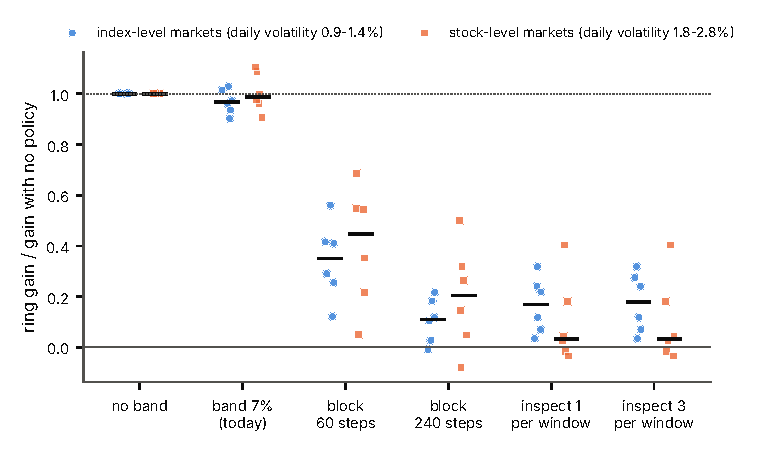
\includegraphics[width=0.95\linewidth]{figures/ensemble.pdf}
\caption{The best-responding ring's gain relative to its gain with no policy, one point per calibrated market and the median as a line. Daily band 7\% in all policies but the first}\label{fig:ensemble}
\end{figure}

\begin{table}[t]
\centering\footnotesize
\adjustbox{max width=\linewidth}{\begin{tabular}{lrrrrr}
\toprule
policy & median gain & range over markets & median ratio to no policy & median detection prob. & deterred at $m=5$ \\
\midrule
no price band & 110.0k & 86.7k to 162.1k & 1.00 & -- & -- \\
band 7\% (HOSE today) & 105.0k & 89.2k to 164.6k & 0.97 & -- & -- \\
band 7\% + block at 60-step mean & 38.4k & 11.7k to 90.8k & 0.35 & -- & -- \\
band 7\% + block at 240-step mean & 15.3k & -0.9k to 23.5k & 0.11 & -- & -- \\
band 7\% + inspect 1 per window & 16.8k & 4.5k to 51.6k & 0.17 & 17\% & 2/6 \\
band 7\% + inspect 3 per window & 16.8k & 4.5k to 51.6k & 0.18 & 42\% & 5/6 \\
\bottomrule
\end{tabular}
}
\caption{Index-level family of six calibrated markets: the best-responding ring's gain (tick-lots) against each policy, the median probability that a member is inspected in some window of an episode, and the number of markets in which the ring's expected net benefit is non-positive at a fine of five times the gain.}\label{tab:ensemble}
\end{table}

\paragraph{Stock-level family.} The case stocks are more volatile than the index, so we repeat the exercise with six markets whose daily volatility is 1.8--2.8\% (Table~\ref{tab:ensemblestock}; same ring strategy set, not re-optimised). The ring's gain with no policy is larger (median 164k against 110k at index level). The conclusions on the band and on inspection are unchanged in sign: the band leaves the gain at a median 99\% of its value. Under inspection the best-responding ring shrinks its operation: its median gain falls to 3\% of the no-policy gain (6k), with a median probability of being caught of 8\% with one inspected account per window and 25\% with three. The ring's expected net benefit at $m=5$ is non-positive in three of six markets with one inspected account and in five of six with three; in the remaining market with one inspected account the ring still nets up to 41k, and with three up to 7k. The detection probabilities are lower than at index level, where each window has fewer accounts to cover, yet deterrence is not worse, because the ring's remaining gain is smaller relative to the fine; we have not separated the two effects. In both families the price band has no effect, block pricing and inspection have large ones, and no single rule removes the ring's gain in every market.

\begin{table}[t]
\centering\footnotesize
\adjustbox{max width=\linewidth}{\begin{tabular}{lrrrrr}
\toprule
policy & median gain & range over markets & median ratio to no policy & median detection prob. & deterred at $m=5$ \\
\midrule
no price band & 164.4k & 101.2k to 261.4k & 1.00 & -- & -- \\
band 7\% (HOSE today) & 154.9k & 111.9k to 261.1k & 0.99 & -- & -- \\
band 7\% + block at 60-step mean & 66.5k & 8.4k to 179.0k & 0.45 & -- & -- \\
band 7\% + block at 240-step mean & 33.7k & -7.9k to 131.0k & 0.20 & -- & -- \\
band 7\% + inspect 1 per window & 6.3k & -9.1k to 40.8k & 0.03 & 8\% & 3/6 \\
band 7\% + inspect 3 per window & 6.3k & -9.1k to 40.8k & 0.03 & 25\% & 5/6 \\
\bottomrule
\end{tabular}
}
\caption{Stock-level family of six calibrated markets (daily volatility 1.8--2.8\%): the ring's gain against each policy, as in Table~\ref{tab:ensemble}.}\label{tab:ensemblestock}
\end{table}

\subsection{Markets without trending}\label{sec:acf}

\textit{(pending)}

\subsection{The block reference price: law, ex-post evaluation and best response}\label{sec:blockcheck}

Because the reference price enters only the ring's payoff (Section~\ref{sec:blocklaw}), the effect of the rule for every $L$ can be computed exactly from the same simulated episodes. For each market of both families and each of the four strategies we simulate 12 selection and 12 reporting episodes once and score them with $L\in\{1,5,15,30,60,120,240,480\}$. Table~\ref{tab:block} and Figure~\ref{fig:block} report the median over markets. The \emph{block term} is the value of the block alone (block size times credited displacement); the total gain adds trading profit, which the rule does not touch. The rule removes most of the block term: a reference of 60 steps leaves 42\% (index level) and 39\% (stock level) of it, a one-day reference 13\% and 2\%. The linear-ramp law of Proposition~\ref{prop:block}, with the measured push duration $a=72$ to $83$ steps, has the right shape and order of magnitude but overstates the retained value at $L\ge30$ (0.61 against 0.42 at $L=60$ at index level, 0.16 against 0.13 at $L=240$), because the real price path is not a ramp ending at the sale. The total gain falls to a median 52\% (60 steps) and 28\% (240 steps) of its value at index level and to 69\% and 44\% at stock level, as the trading profit remains; with a reference of two days ($L=480$) the median total gain is about zero ($-0.03$ at index level, $0.12$ at stock level), and in markets where the unconstrained gain is small the ring loses money already at 60 to 240 steps. Re-selecting the strategy (``adaptive'') changes the median only slightly: within the four strategies the ring finds no good counter, and the gap between the adaptive and the static curve is the value of adaptation. The independent episodes of the earlier ensemble run (Table~\ref{tab:ensemble}) give a lower retained share of the total gain (35\% and 11\% at index level, 45\% and 20\% at stock level for 60 and 240 steps); with episode-to-episode standard errors of about a third of the mean in gain, we read the evidence as: a one-day reference leaves the ring between roughly one tenth and one half of its gain, and removes most of the block value.

\paragraph{Sensitivity to the block size.} The block of 3000 lots is an assumption of the simulator, and it matters: the rule acts on the block term only, so its effect on the total gain depends on how much of the gain comes from the block. The size enters only the payoff, so a different size can be evaluated exactly on the same episodes (Appendix~\ref{app:extra}). With a block of 10,000 lots the ring keeps 19--21\% of its gain at a one-day reference; with the assumed size 28--44\%; with a block of 1000 lots 60--64\%, and of 300 lots 83--87\%, because trading profit then dominates. The rule is effective against a ring whose gain is realised through off-book blocks and has no effect on a ring that profits through trading on the book.

\begin{figure}[t]
\centering
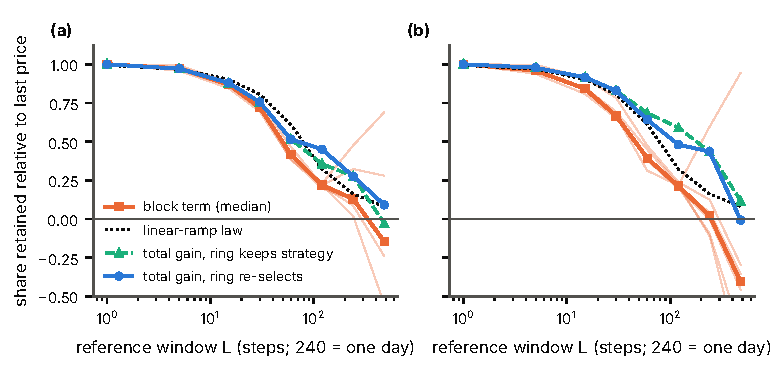
\includegraphics[width=\linewidth]{figures/block.pdf}
\caption{Share of the ring's block term and of its total gain retained against the reference window $L$, for the index-level (a) and stock-level (b) families: median over six markets of the block term (thick orange; thin lines are the six markets), the linear-ramp law of Proposition~\ref{prop:block}, and the total gain for a ring that keeps its strategy and for a ring that re-selects it}\label{fig:block}
\end{figure}

\begin{table}[t]
\centering\scriptsize
\setlength{\tabcolsep}{3pt}
\adjustbox{max width=\linewidth}{\begin{tabular}{lrrrrrrrr}
\toprule
& \multicolumn{4}{c}{index level} & \multicolumn{4}{c}{stock level} \\
\cmidrule(lr){2-5}\cmidrule(lr){6-9}
$L$ & block term & law & total, static & total, adaptive & block term & law & total, static & total, adaptive \\
\midrule
15 & 0.87 & 0.90 & 0.88 & 0.88 & 0.84 & 0.90 & 0.91 & 0.91 \\
30 & 0.72 & 0.81 & 0.76 & 0.76 & 0.67 & 0.81 & 0.83 & 0.83 \\
60 & 0.42 & 0.61 & 0.52 & 0.52 & 0.39 & 0.61 & 0.68 & 0.64 \\
120 & 0.22 & 0.32 & 0.36 & 0.45 & 0.21 & 0.32 & 0.59 & 0.48 \\
240 & 0.13 & 0.16 & 0.28 & 0.28 & 0.02 & 0.16 & 0.44 & 0.44 \\
480 & -0.15 & 0.08 & -0.03 & 0.09 & -0.41 & 0.08 & 0.12 & -0.01 \\
\bottomrule
\end{tabular}
}
\caption{Block-price rule, median over six markets per family: share of the block term and of the total gain retained when the block is priced at the mean of the last $L$ steps instead of the last price, and the prediction of the linear-ramp law.}\label{tab:block}
\end{table}

\subsection{Inspection capacity and the deterrence frontier}\label{sec:frontier}

Proposition~\ref{prop:deter} turns the power law into a capacity requirement. With the constants fitted in Section~\ref{sec:powercheck} ($s_0=1.20$), Table~\ref{tab:capacity} gives the number of accounts that must be inspected per window to deter a ring of three accounts active in four windows, and the saving over random inspection. In a market with 600 active accounts per window, screening deters at a fine of five times the gain with about 3 inspected accounts per window (0.5\% of accounts) against 11 for random inspection, and at ten times with 1.2 against 5.2; doubling the fine multiple therefore saves a factor of about 2.4 in capacity, which gives the regulator two exchangeable instruments (Section~\ref{sec:discussion}). The advantage of screening shrinks as the market grows (saving of 3.7 at 600 accounts and 2.0 at 2000). The model's detection probability for a ring of three accounts in four windows with one and three inspected accounts (8\% and 20\%) is close to the probability found for the best-responding ring in the stock-level family (8\% and 25\%) and below that of the index-level family (17\% and 42\%; Figure~\ref{fig:frontier}a). We do not know which sizes the best-responding ring chose, so this agreement is suggestive, not a test.

\begin{figure}[t]
\centering
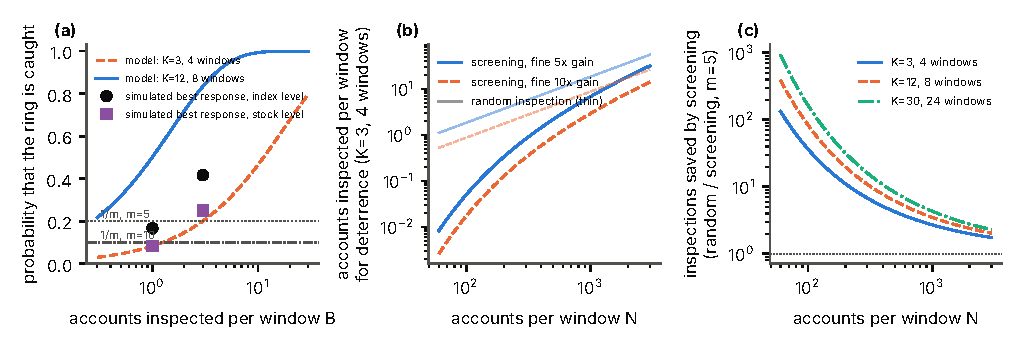
\includegraphics[width=\linewidth]{figures/frontier.pdf}
\caption{Deterrence frontier. (a) Probability that the ring is caught against the number of inspected accounts per window at $N=600$ for two ring sizes (model, solid and dashed), with the thresholds $1/m$ for $m=5,10$ (horizontal lines) and the median probability of the best-responding ring in the two simulated families (points). (b) Accounts to inspect per window for deterrence of a ring of three accounts active in four windows against $N$, by screening (thick) and by random inspection (thin). (c) Inspections saved by screening against $N$ for three ring sizes and activity levels, fine five times the gain}\label{fig:frontier}
\end{figure}

\begin{table}[t]
\centering\footnotesize
\adjustbox{max width=\linewidth}{\begin{tabular}{lrrrrrr}
\toprule
& \multicolumn{3}{c}{fine $5\times$ gain} & \multicolumn{3}{c}{fine $10\times$ gain} \\
\cmidrule(lr){2-4}\cmidrule(lr){5-7}
$N$ & screening & random & saving & screening & random & saving \\
\midrule
100 & 0.05 & 1.8 & 36.5 & 0.02 & 0.9 & 50.2 \\
300 & 0.81 & 5.5 & 6.8 & 0.32 & 2.6 & 8.1 \\
600 & 2.99 & 11.1 & 3.7 & 1.25 & 5.2 & 4.2 \\
1000 & 6.81 & 18.4 & 2.7 & 2.93 & 8.7 & 3.0 \\
2000 & 18.48 & 36.8 & 2.0 & 8.17 & 17.5 & 2.1 \\
\bottomrule
\end{tabular}
}
\caption{Inspected accounts per window needed to deter a ring of three accounts active in four windows (Proposition~\ref{prop:deter} with $s_0=1.20$): by screening and by random inspection, and the saving, for fine multiples 5 and 10.}\label{tab:capacity}
\end{table}

\subsection{Other manipulation types and the cost to honest investors}

Table~\ref{tab:matrix} and Figure~\ref{fig:tradeoff} report, for the first calibrated market, what a fixed spoofer, pump-and-dump agent, wash pair and ring achieve under order-level rules and what the rules cost honest participants. In this market, minimum resting times and cancel fees do not reduce what the manipulators achieve: spoofing profit is 872 (s.e.\ 125) with no rule and 1,091 to 1,380 with minimum resting times or fees, and the spoofing price impact is higher, not lower, with a longer minimum resting time (0.26 against 0.11 ticks); pump impact is lower under cancel fees (0.31 against 0.47, within about 1.3 standard errors); wash volume is 3.3\% of volume under every rule, and the ring's gain is unaffected except by the block price. These rules cost honest investors: a minimum resting time of 15 steps raises the spread by 7\% and volatility by 21\%, and a cancel fee of 2 raises volatility by 24\%. A tick twice as large widens the spread by 35\% and cuts depth by 10\% while lowering spoofing profit (491 against 872). The block price rule has no effect on honest trading in this experiment because honest agents do not trade blocks; its cost is the gap between the last price and the trailing mean, 0.17\% of price at 60 steps and 0.50\% at 240 steps in the first preset.

\begin{figure}[t]
\centering
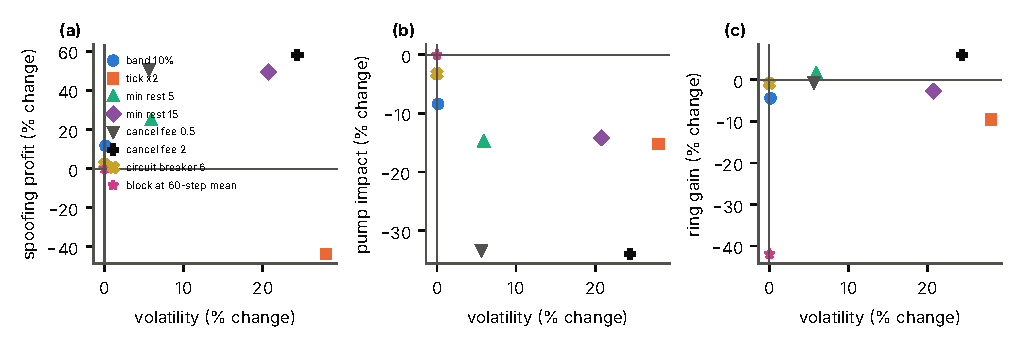
\includegraphics[width=\linewidth]{figures/tradeoff.pdf}
\caption{Effect on manipulators against cost to honest participants, first calibrated market. Each point is an order-level rule or band setting; the horizontal axis is the change of the honest-only volatility, the vertical axis the change in (a) spoofing profit, (b) pump impact and (c) ring gain, relative to the market with a 7\% band and no other rule. Manipulators do not adapt}\label{fig:tradeoff}
\end{figure}

\begin{table}[t]
\centering\scriptsize
\setlength{\tabcolsep}{3pt}
\adjustbox{max width=\linewidth}{\begin{tabular}{lrrrrrrrrr}
\toprule
policy & spread & depth & volatility & retail cost & volume & spoof impact & pump impact & wash share & ring gain \\
\midrule
band 7\% (today) & +0\% & +0\% & +0\% & +0\% & +0\% & 0.11 & 0.47 & 0.033 & 34k \\
band 10\% & -0\% & -0\% & +0\% & -2\% & -0\% & 0.14 & 0.43 & 0.033 & 32k \\
tick x2 & +35\% & -9\% & +28\% & -16\% & +7\% & 0.21 & 0.40 & 0.031 & 30k \\
min rest 5 & +2\% & -1\% & +6\% & -5\% & -0\% & 0.16 & 0.40 & 0.033 & 34k \\
min rest 15 & +7\% & -3\% & +21\% & -12\% & +1\% & 0.26 & 0.40 & 0.032 & 33k \\
cancel fee 0.5 & +2\% & -2\% & +6\% & -5\% & +1\% & 0.18 & 0.31 & 0.032 & 33k \\
cancel fee 2 & +8\% & -6\% & +24\% & -5\% & +5\% & 0.20 & 0.31 & 0.031 & 36k \\
circuit breaker 6 & -0\% & -0\% & -0\% & +1\% & -0\% & 0.15 & 0.45 & 0.033 & 33k \\
block at 60-step mean & +0\% & +0\% & +0\% & +0\% & +0\% & 0.11 & 0.47 & 0.033 & 20k \\
\bottomrule
\end{tabular}
}
\caption{First calibrated market, 10 honest-only and 24 manipulated episodes per policy. Spread, depth, volatility, retail trading cost and volume are relative to the band-7\% market; spoofing and pump impact are in ticks; ``wash share'' is the share of volume traded between colluding accounts; ring gain is in tick-lots. Manipulators do not adapt. Retail cost includes fees paid; it falls under larger ticks and fees because simulated noise traders mostly post passive orders and earn the spread.}\label{tab:matrix}
\end{table}

\subsection{Checking a lever against reality: the 2016 tick-size reform}\label{sec:tick}

The tick size is the one lever in the simulator for which a real natural experiment is available in public data. On 12 September 2016 the Ho Chi Minh Stock Exchange reduced its minimum tick (to 10, 50 and 100 VND below 10,000, between 10,000 and 49,950, and above 50,000 VND), while HNX and UPCoM stocks were not affected \citep[according to][]{vo2023}. Using daily open, high, low, close and volume, we compare 282 HOSE stocks with 489 control stocks over the 40 trading days before and the 40 days from one week after the reform. Outcomes are the Corwin--Schultz high-low spread estimator, the daily range, the absolute return, the share of zero-return days and log volume. We could not establish the old tick from our sources (one summary gave 500 VND for all prices, which cannot be right given the small observed spread change), so we compare with simulated reductions of the tick by factors of 2, 5 and 10.

Table~\ref{tab:tickcompare} and Figure~\ref{fig:tick} show the result. The share of zero-return days fell by 7.1 points relative to controls (95\% interval $-9.2$ to $-5.0$), by 8.3 points with 20-day windows and by 6.7 with 60-day windows, a larger change than in any of four placebo dates; the spread estimate fell by 0.06 points (8\% of its pre-reform level; interval $-0.13$ to $0.01$), and by 0.07 points with 60-day windows, with placebo estimates ranging from $-0.06$ to $+0.09$. By price tercile the fall in the spread estimate is concentrated in low-priced stocks ($-0.18$ points, interval $-0.32$ to $-0.03$, against a pre-reform level of 1.0\%). The simulator predicts a fall of the share of zero-return days by 38\% for a halving of the tick, 43\% for a five-fold cut and 78\% for a ten-fold cut (real: 24\%), and of the spread estimate by 21\%, 65\% and 85\% (real: 8\%). The signs agree, in line with the finding of lower trading costs by \citet{vo2023} on intraday data; the real effect is of the order of the simulator's prediction for a halving of the tick and much smaller than for a five- or ten-fold cut. Prices in the panel are adjusted, so price bands are approximate, and the design cannot separate the reform from other changes on HOSE in the same weeks.

\begin{figure}[t]
\centering
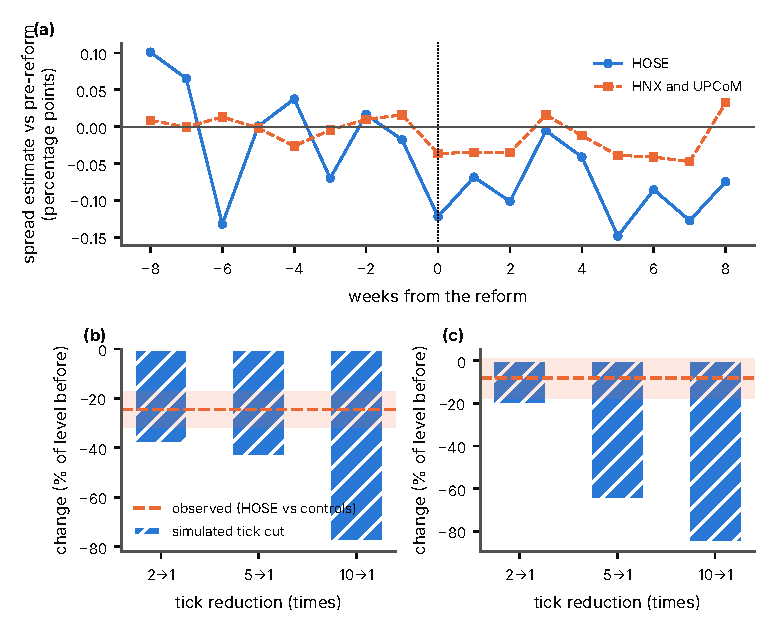
\includegraphics[width=\linewidth]{figures/tick.pdf}
\caption{The 2016 tick reform. (a) Weekly change of the Corwin--Schultz spread estimate relative to the 40 days before the reform for 282 HOSE stocks and 489 controls. (b), (c) Simulated change after a tick reduction by a factor of 2, 5 and 10 (bars) against the observed difference-in-differences (dashed line, shaded 95\% interval), as a percentage of the level before, for the share of zero-return days (b) and the spread estimate (c)}\label{fig:tick}
\end{figure}

\begin{table}[t]
\centering\scriptsize
\setlength{\tabcolsep}{3pt}
\adjustbox{max width=\linewidth}{\begin{tabular}{lccccc}
\toprule
outcome & real DiD (95\% interval) & real, relative to HOSE pre-period level & sim: tick $2\to1$ & $5\to1$ & $10\to1$ \\
\midrule
CS spread (\%) & -0.061 [-0.133, 0.008] & -8\% & -21\% & -65\% & -85\% \\
daily range (\%) & -0.067 [-0.213, 0.116] & -2\% & -7\% & -31\% & -50\% \\
|return| (\%) & -0.141 [-0.270, 0.012] & -8\% & -3\% & -35\% & -44\% \\
zero-return share & -0.071 [-0.092, -0.050] & -24\% & -38\% & -43\% & -78\% \\
log volume & -0.000 [-0.153, 0.172] & -- & -- & -- & -- \\
\bottomrule
\end{tabular}
}
\caption{Tick-size reform: real difference-in-differences against the simulator's prediction for a reduction of the tick by a factor of 2, 5 or 10. Changes relative to the pre-reform level.}\label{tab:tickcompare}
\end{table}

\subsection{Summary of the policy evidence}

Table~\ref{tab:summary} lists, for each lever, what the simulated markets and the real data show.

\begin{table}[t]
\centering\footnotesize
\begin{adjustbox}{max width=\linewidth}
\begin{tabular}{p{3.1cm}p{4.2cm}p{3.6cm}p{3.6cm}}
\toprule
lever & against rings & against spoofing, pumps, wash & cost to honest investors\\
\midrule
inspection with a fine proportional to the gain & deters with enough capacity (three accounts per window: 5 of 6 markets in each family); capacity falls by a factor of 2.4 when the fine multiple doubles & not tested & fine paid by manipulators only; inspection effort\\
off-book block priced at a trailing mean & removes 58--61\% of the block value at 60 steps and 87--98\% at one day; total gain falls to 28--44\% of its value at one day (block of 3000 lots; Appendix~\ref{app:extra}) & not applicable & 0.17\%--0.50\% of price on block trades\\
daily price band 7\% or 10\% & no effect in the markets tested & not tested & none observed in honest markets\\
minimum resting time, cancel fee & no effect & no reduction; spoofing profit and impact not lower & volatility +6\% to +24\%, spread up to +8\%\\
tick size & not tested for rings & larger tick lowers spoofing profit & spread +35\% for a doubled tick; real tick cut improved liquidity\\
\bottomrule
\end{tabular}
\end{adjustbox}
\caption{Policy evidence in this paper (simulated markets calibrated to Vietnam unless stated; the tick row also uses real data).}\label{tab:summary}
\end{table}
